\documentclass{article}
\usepackage{graphicx}

\begin{document}

\begin{center}


\includegraphics[width=5cm]{IMG_20260310_120019.jpg}

\vspace{0.5cm}

Name: Keshava Reddy V \\ 
ID: COMETFWC054

\vspace{0.5cm}

{\Large \textbf{GATE CS 2010}}

\end{center}

\section*{Question 6}

The minterm expansion of  

$f(P,Q,R) = PQ + QR + PR$

\begin{enumerate}
\item $m_2 + m_4 + m_6 + m_7$
\item $m_0 + m_1 + m_3 + m_5$
\item $m_0 + m_1 + m_6 + m_7$
\item $m_2 + m_3 + m_4 + m_5$
\end{enumerate}

\section*{Question Analysis}

Given function:

$f(P,Q,R) = PQ + QR + PR$

\begin{itemize}
\item This is a 3-input majority function.
\item Output becomes 1 when at least two inputs are 1.
\end{itemize}

\section*{Truth Table}

\begin{center}

\begin{tabular}{|c|c|c|c|}
\hline
P & Q & R & F \\
\hline
0 & 0 & 0 & 0 \\
0 & 0 & 1 & 0 \\
0 & 1 & 0 & 0 \\
0 & 1 & 1 & 1 \\
1 & 0 & 0 & 0 \\
1 & 0 & 1 & 1 \\
1 & 1 & 0 & 1 \\
1 & 1 & 1 & 1 \\
\hline
\end{tabular}

\end{center}

\section*{Python Code}

\begin{verbatim}
import numpy as np
import matplotlib.pyplot as plt

P = np.array([0,0,0,0,1,1,1,1])
Q = np.array([0,0,1,1,0,0,1,1])
R = np.array([0,1,0,1,0,1,0,1])

F = (P & Q) | (Q & R) | (P & R)
\end{verbatim}

\section*{Graph}

\begin{center}

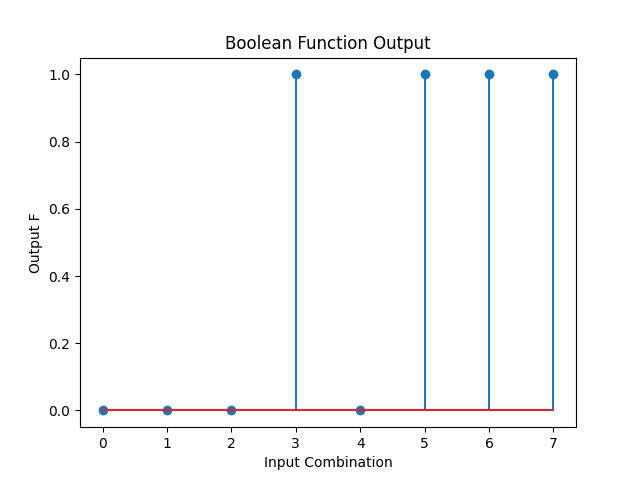
\includegraphics[width=10cm]{kmap_graph.png}

\end{center}

\section*{Conclusion}

The function produces output 1 when at least two inputs are 1.

The minterm expansion is:

$m_3 + m_5 + m_6 + m_7$

\end{document}
